\chapter{Introduction}


\section{Data Communications}
The word data refers to information presented in whatever form is agreed upon by the parties creating and using the data. Data communications are the exchange of data between two devices via some form of transmission medium such as a wire cable.

\subsection{Components}
A data communications system has five components:

\begin{enumerate}[itemsep=1ex]
   \item \textbf{Message:} The message is the information (data) to be communicated by the sender to the receiver.
   
   \item \textbf{Sender:} The sender is the device that sends the data (message).
   
   \item \textbf{Receiver:} The receiver is the device that receives the message.
   
   \item \textbf{Transmission medium:} The transmission medium is the physical path by which a message travels from sender to receiver. E.g: twisted-pair cable, radio waves.
   
   \item \textbf{Protocol:} A protocol is a set of rules that govern data communications. It represents an agreement between the communicating devices. Without a protocol, two devices may be connected but not communicating.
\end{enumerate}

\begin{figure}[th]
   \centering
   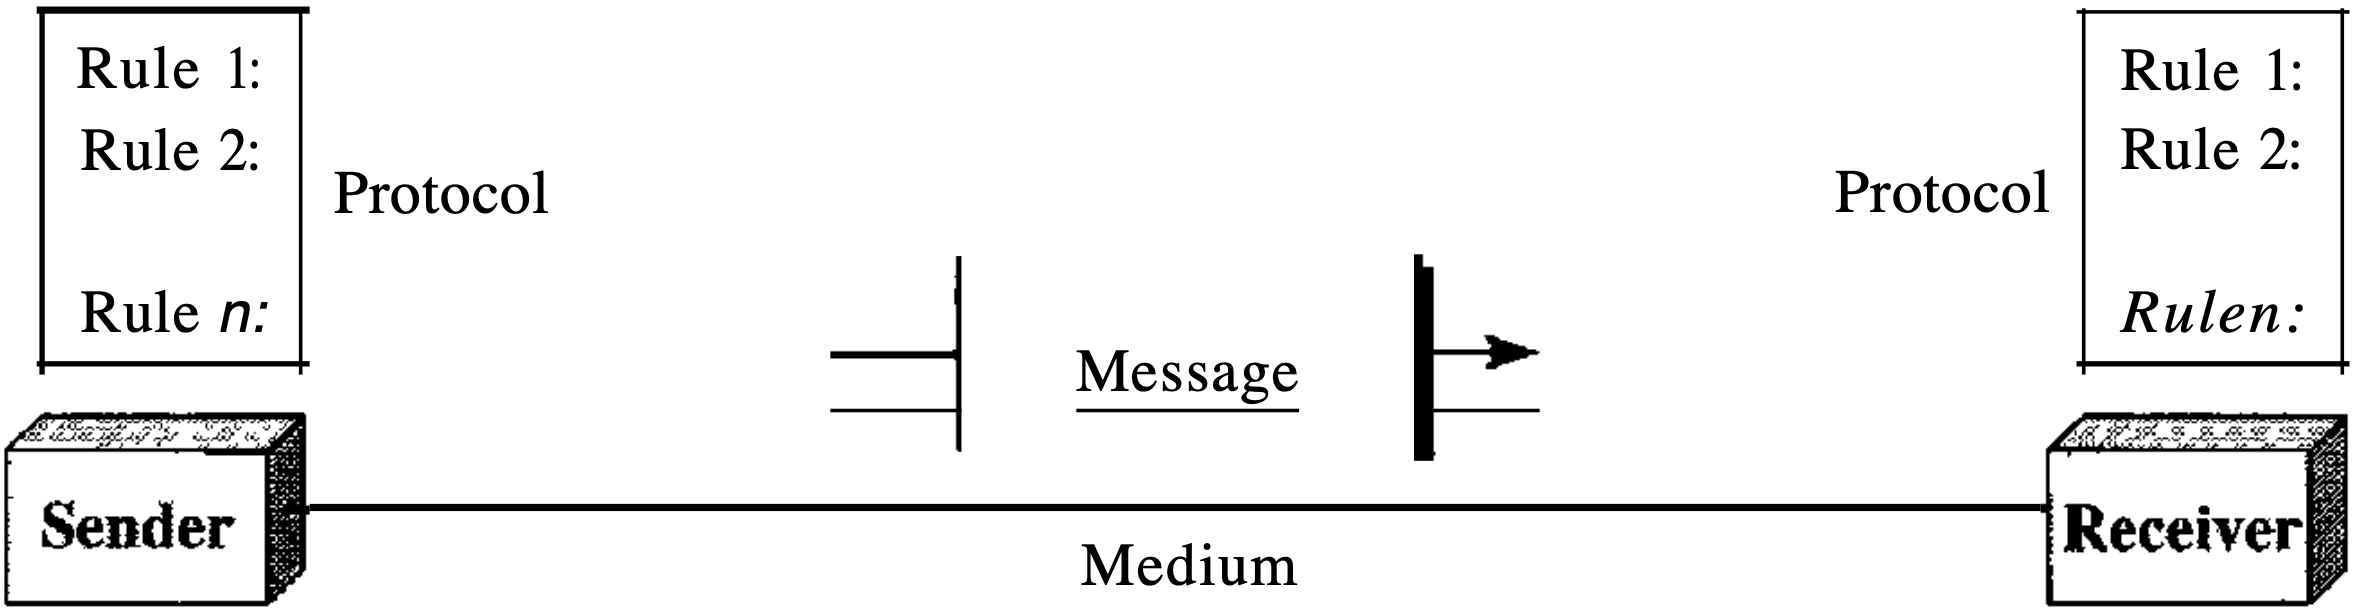
\includegraphics[width=10cm]{figures/Data Communication Components.JPG}
   \caption{Five components of data communication}
\end{figure}

\section{Characteristics of a Data Communication System}
\begin{itemize}
    \item \textbf{Delivery:} Ensures that the message reaches the correct destination in a timely manner.
    \item \textbf{Accuracy:} Data should be transmitted without errors, preserving the integrity of the message during transmission.
    \item \textbf{Timeliness:} Data must be delivered within a specified time frame, particularly for time-sensitive applications like real-time systems (e.g., video conferencing).
    \item \textbf{Jitter:} Refers to the variation in packet arrival times. Inconsistent delays can degrade performance, particularly in real-time systems.
    \item \textbf{Security:} Measures are taken to protect data from unauthorized access, modification, or destruction.
    \item \textbf{Scalability:} The system should be able to accommodate an increasing number of users, devices, and data without degrading performance.
    \item \textbf{Synchronization:} Some applications, such as video streaming, require the continuous and synchronized delivery of data.
    \item \textbf{Error Detection and Correction:} Mechanisms should be in place to identify and correct errors that occur during transmission.
\end{itemize}

\pagebreak
\subsection{Data flow}
Communication between two devices can be simplex, half-duplex, or full-duplex.

\begin{tabularx}{\textwidth}{|L|L|L|L|}\hline
   \textbf{Comparison} &
   \textbf{Simplex} &
   \textbf{Half-Duplex} &
   \textbf{Full-Duplex} \\\hline
   
   Direction of Communication &
   One-way only (unidirectional) &
   Two-way, but one at a time (alternating) &
   Two-way simultaneously (bi-directional) \\\hline

   Send / Receive	&
   Can only send (transmit) or only receive &
   Send and receive, but not at the same time &
   Send and receive at the same time \\\hline

   Performance &
   Lower performance, limited to single direction &
   Moderate performance, switching between send/receive &
   High performance, simultaneous communication \\\hline

   Example &
   Keyboard, Radio &
   Walkie-talkie &
   Telephone, modern internet connection \\\hline
\end{tabularx}


% \section{Network}
% A network is a set of devices (often referred to as \textbf{nodes}) connected by communication \textbf{links}. A node can be a computer, printer, or any other device capable of sending and/or receiving data generated by other nodes on the network. A link can be a cable, air, optical fiber, or any medium which can transport a signal carrying information.

% \subsection{Network Criteria}
% A network must be able to meet a certain number of criteria. The most important of these are performance, reliability, and security.
% \begin{itemize}
%    \item \textbf{Performance:} 
%    Performance depends on the factors of network a elements. Often evaluated by two networking metrics: throughput and delay. If we try to send more data to the network, we may increase throughput but we increase the delay because of traffic congestion in the network.

%    \item \textbf{Reliability:} 
%    Network reliability is measured by the frequency of failure, the time it takes a link to recover from a failure, and the network's robustness in a catastrophe.

%    \item \textbf{Security:}  
%    Network security issues include protecting data from unauthorized access, protecting data from damage and development, and implementing policies and procedures for recovery from breaches and data losses.
% \end{itemize}

% \section{Physical Structures}
% A network is two or more devices connected through links. A link is a communications pathway that transfers data from one device to another. For communication to occur, two devices must be connected in some way to the same link at the same time. There are two possible types of connections: point-to-point and multipoint.

% \subsection{Point-to-Point}
% A point-to-point connection provides a dedicated link between two devices. The entire capacity of the link is reserved for transmission between those two devices.

% \subsection{Multipoint}
% A multipoint (also called multidrop) connection is one in which more than two specific devices share a single link. In a multipoint environment, the capacity of the channel is shared, either spatially or temporally.

\section{Network Topology}
A network topology is the geometric representation of the relationship of all the links and linking devices (usually called nodes) to one another. There are four basic topologies possible: Mesh, Star, Bus, and Ring.

\begin{tabularx}{\textwidth}{|p{2.5cm}|L|L|L|L|}
   \hline
   \textbf{Feature} & \textbf{Mesh} & \textbf{Star} & \textbf{Bus} & \textbf{Ring} \\
   \hline
   \textbf{Structure} & Every device is connected to every other device & All devices are connected to a central hub or switch & All devices are connected to a single central cable & Devices are connected in a circular fashion \\
   \hline
   \textbf{Transmission Mode} & Full-duplex & Half-duplex & Half-duplex & Half-duplex \\\hline
   \textbf{Type of Link} & Point-to-point & Point-to-point & Multipoint & Point-to-point \\\hline
   \textbf{Number of Links} & $\frac{n(n-1)}{2}$ link \newline (for a full mesh) & $n$ link (each device has 1 connection to the hub) & 1 link (shared bus) & $n$ links (one link per device to its neighbor) \\\hline
   \textbf{Key Device} & Switch & Hub or Switch & Terminators & Token-Passing Device \\\hline

   \textbf{Robustness} &
   Very high (multiple paths for redundancy) &
   Moderate (depends on the central hub) &
   Low (failure of the bus affects all devices) &
   Low (failure of one link can break the ring) \\\hline

   \textbf{Security} &
   High; data can be sent directly between devices &
   Moderate; data passes through central hub &
   Low; data is shared across a single bus &
   Moderate; data passes through each device 
   \\\hline

   \textbf{Scalability} & High; can be expanded easily by adding more connections & Moderate; easy to add devices but requires more hubs or switches & Low; adding devices can affect network performance & Low; adding devices requires breaking the ring \\
   \hline
   \textbf{Performance} & High; multiple paths, no congestion & High; central hub reduces congestion & Lower; performance due to data collisions & Moderate; performance may degrade as devices are added \\
   \hline
   \textbf{Installation Cost} & High; requires many cables and connections & Moderate; cost of hub/switch and cables & Low; minimal cabling required & Low to Moderate; less cabling than mesh \\
   \hline
   \textbf{Maintenance} & Complex; difficult to manage due to many connections & Simple; centralized management through hub & Simple; less cabling but network troubleshooting can be challenging & Troubleshooting can be complex due to circular connections \\
   \hline
\end{tabularx}

\section{Networking Devices}
\begin{tabularx}{\textwidth}{|X|X|X|X|}
   \hline
   \textbf{Topic} & \textbf{Hub} & \textbf{Switch} & \textbf{Router} \\
   \hline
   OSI Layer & Physical Layer (Layer 1) & Data Link Layer (Layer 2) & Network Layer (Layer 3) \\
   \hline
   Function & Broadcasts data to all devices & Forwards data to a specific device & Routes data between different networks \\
   \hline
   Data Transmission form & Electrical signals (bits) & Frames & Packets \\
   \hline
   No. of Ports & 4 to 24 ports & 24 to 48 ports & 2 to 8 ports (or more in enterprise) \\
   \hline
   Transmission type & Broadcast & Unicast, Multicast, Broadcast & Unicast \\
   \hline
   Device type & Passive device & Intelligent device & Intelligent device \\
   \hline
   Used in (LAN, MAN, WAN) & LAN & LAN & LAN, MAN, WAN \\
   \hline
   Transmission mode & Half-duplex & Full-duplex & Full-duplex \\
   \hline
   Speed & 10 Mbps & 10/100/1000 Mbps & Varies (depends on WAN links, e.g., 1 Gbps) \\
   \hline
\end{tabularx}

\section{Area Network}
\begin{table}[th]
   \begin{tabularx}{\textwidth}{|l|L|L|L|}
      \hline
      \textbf{Aspect} &
      \textbf{LAN} &
      \textbf{MAN} &
      \textbf{WAN} \\\hline

      \textbf{Geographical Coverage} &
      Small area (within a building or a campus) &
      Medium area (citywide or metropolitan area) &
      Very large area (countrywide or global) \\\hline

      \textbf{Data Transfer Rate} &
      High-speed &
      Moderate (higher than WAN) &
      Relatively slower than LAN \\\hline

      \textbf{Latency} &
      Low latency due to close proximity of devices &
      Moderate latency, depending on the size of the network &
      Higher latency due to distance and routing through multiple networks \\\hline

      \textbf{Cost} &
      Relatively low setup and maintenance costs &
      High setup and operational costs due to long-distance infrastructure &
      Moderate cost, as it requires more infrastructure than LAN but less than WAN \\\hline

      \textbf{Ownership} &
      The ownership of LAN is private &
      The ownership of MAN might be public or private &
      The ownership of WAN might be private or public \\\hline
   \end{tabularx}
\end{table}


\begin{figure}[th]
   \centering
   \begin{subfigure}{\textwidth}
      \centering
      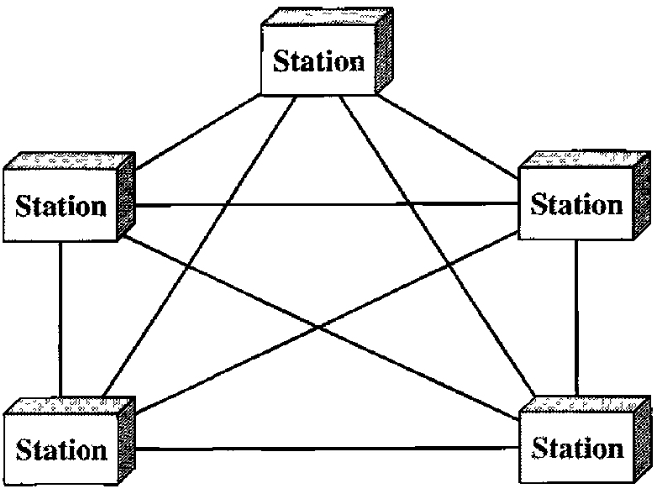
\includegraphics[width=7cm]{figures/Mesh topology.JPG}
      \caption{Mesh topology}
   \end{subfigure}
   
   \vspace{12ex}
   \begin{subfigure}{\textwidth}
      \centering
      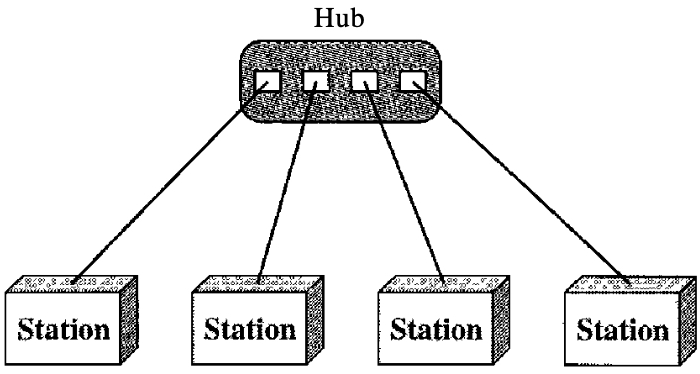
\includegraphics[width=7cm]{figures/Star topology.JPG}
      \caption{Star topology}
   \end{subfigure}
   
   \vspace{12ex}
   \begin{subfigure}{\textwidth}
      \centering
      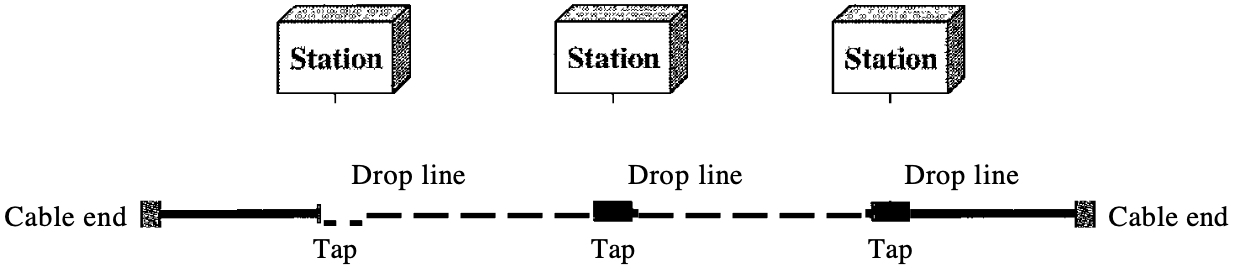
\includegraphics[width=14cm]{figures/Bus topology.JPG}
      \caption{Bus topology}
   \end{subfigure}
   
   \vspace{12ex}
   \begin{subfigure}{\textwidth}
      \centering
      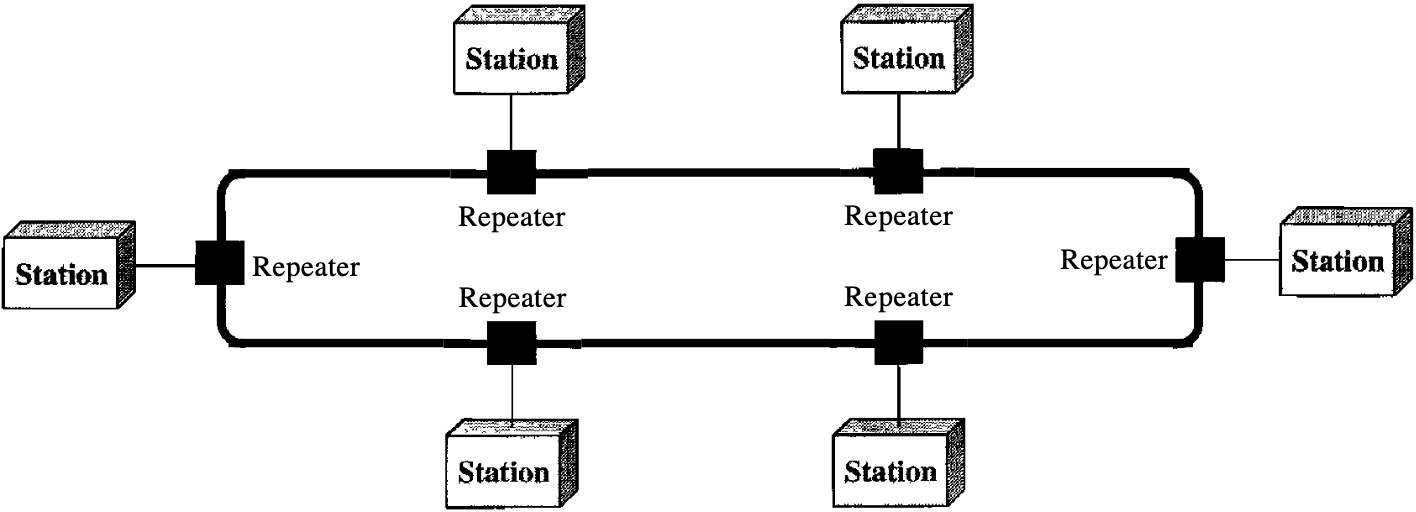
\includegraphics[width=14cm]{figures/Ring topology.JPG}
      \caption{Ring topology}
   \end{subfigure}
\end{figure}


